\section{Difa Al Fansha}

\subsection{Teori}
	%%Nomor 1
	\subsubsection{Kenapa file teks harus di lakukan tokenizer}
	\hfill\\
	%%Jawaban Nomor 1
Untuk memudahkan mesin memahami maksud dari apa yang kita inginkan dalam 
machine learning, kata pada teks disebut token, dan proses vektorisasi dari bentuk
kata ke dalam token tersebut disebut tokenizer dan tokenizer akan merubah sebuah
teks menjadi simbol, kata, ataupun biner dan bentuk lainnya kedalam token. Untuk lebih jelasnya perhatikan ilustrasi berikut. Disini saya mempunyai sebuah kalimat yaitu ”Nama Saya Difa Al Fansha” maka ketika kita lakukan proses tokenizer
maka akan berubah menjadi [’Nama’, ’Saya’, 'Difa', 'Al', 'Fansha']

	\begin{figure}[H]
		\begin{center}
		 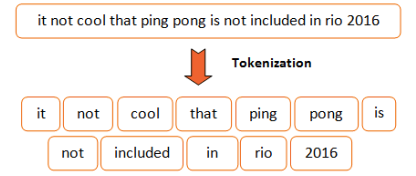
\includegraphics[width=10cm]{figures/1174076/figures7/teori1.png}
		 \caption{Soal 1}	
		\end{center}
	\end{figure}

	%%Nomor 2
	\subsubsection{konsep dasar K Fold Cross Validation pada dataset komentar Youtube pada kode listing 7.1.}
	\hfill\\
	%%Jawaban Nomor 2
StartifiedKFold berisikan presentasi sampel untuk setiap kelas. Dimana dalam
ilustrasi ini sampel dibagi menjadi 5 dalam setiap class nya. Kemudian sampel tadi
akan dimasukan kedalam class dari dataset youtube tadi.	

	 
	%%Nomor 3
	\subsubsection{Apa maksudnya kode program for train, test in splits}
	\hfill\\
	%%Jawaban Nomor 3
Menguji apakah setiap data pada dataset sudah di split dan
tidak terjadi penumpukan. Yang dimana maksudnya di setiap class tidak akan muncul
id yang sama. Ilustrasinya misalkan kita memiliki 4 baju dengan model yang berbeda.
Kemudian kita bagikan kedua anak, tentunya setiap anak yang menerima baju tidak
memiliki baju yang sama modelnya.

	\begin{figure}[H]
		\begin{center}
		 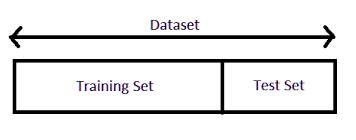
\includegraphics[width=10cm]{figures/1174076/figures7/teori3.png}
		 \caption{Nomor 3}	
		\end{center}
	\end{figure}

	%%Nomor 4
	\subsubsection{Apa maksudnya kode program train content = d[’CONTENT’].iloc[train idx] dan test content = d[’CONTENT’].iloc[test idx]}
	\hfill\\
	%%Jawaban
Mengambil data pada kolom atau index CONTENT yang merupakan bagian dari train idx dan test idx. Ilustrasinya, ketika data telah diubah menjadi train dan test maka kita dapat memilihnya untuk ditampilkan pada kolom yang
diinginkan.


	\begin{figure}[H]
		\begin{center}
		 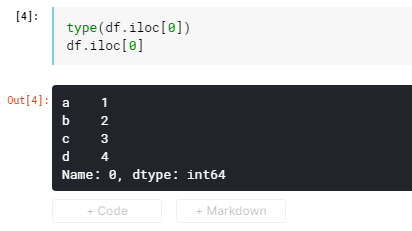
\includegraphics[width=10cm]{figures/1174076/figures7/teori4.png}
		 \caption{Nomor 4}	
		\end{center}
	\end{figure}
	

	%%Nomor 5
	\subsubsection{Apa maksud dari fungsi tokenizer = Tokenizer(num words=2000) dan tokenizer.fit on texts(train content)} 
	\hfill\\
	%%Jawaban
Dimana variabel tokenizer akan melakukan vektorisasi kata menggunakan fungsi
Tokenizer yang dimana jumlah kata yang ingin diubah kedalam bentuk token adalah
2000 kata. Dan untuk tokenizer.fit on texts(train content) maksudnya kita akan melakukan
fit tokenizer hanya untuk dat trainnya saja tidak dengan data test nya untuk kolom
CONTENT. Ilustrasinya, Jadi, jika Anda memberikannya sesuatu seperti, ”Kucing
itu duduk di atas tikar.” Ini akan membuat kamus s.t. word index [”the”] = 0;
word index [”cat”] = 1 itu adalah kata -¿ kamus indeks sehingga setiap kata mendapat nilai integer yang unik.
	
	%%Nomor 6
	\subsubsection{Apa maksud dari fungsi d train inputs = tokenizer.texts to matrix(train content, mode=’tfidf ’) dan d test inputs = tokenizer.texts to matrix(test content, mode=’tfidf ’)}
	\hfill\\
	%%Jawaban
variabel d train inputs akan melakukan tokenizer dari bentuk
teks ke matrix dari data train content dengan mode matriksnya yaitu tfidf begitu juga
dengan variabel d test inputs untuk data test. Berikut gambar ilustrasinya

	%%Nomor 7
	\subsubsection{Apa maksud dari fungsi d train inputs = d train inputs/np.amax(np.absolute(d train inputs)) dan d test inputs = d test inputs/np.amax(np.absolute(d test inputs))}
	\hfill\\
	%%Jawaban
Fungsi np.amax adalah nilai Maksimal. Jika sumbu tidak ada, hasilnya adalah nilai skalar. Jika sumbu diberikan, hasilnya adalah array dimensi a.ndim - 1.

	%%Nomor 8
	\subsubsection{Apa maksud fungsi dari d train outputs = np utils.to categorical(d[’CLASS’].iloc[train idx]) dan d test outputs = np utils.to categorical(d[’CLASS’].iloc[test idx]) dalam kode program}
	\hfill\\
	%%Jawaban
Fungsi dari baris kode tersebut ialah membuat train outputs dengan kategori dari class lalu dengan ketentuan iloc train idx. Kemudian membuat keluaran sebagai output.
	

	%%Nomor 9
	\subsubsection{Apa maksud dari fungsi di listing 7.2.}
	\hfill\\
	%%Jawaban
Fungsi dari baris kode tersebut ialah model perlu mengetahui bentuk input apa yang harus diharapkan. Untuk alasan ini, lapisan pertama dalam model Sequential (dan hanya yang pertama, karena lapisan berikut dapat melakukan inferensi bentuk otomatis) perlu menerima informasi tentang bentuk inputnya.

	%%Nomor 10
	\subsubsection{Apa maksud dari fungsi di listing 7.3 dengan parameter tersebut}
	\hfill\\
	%%Jawaban
Fungsi dari baris kode tersebut ialah bisa meneruskan nama fungsi loss yang ada, atau melewati fungsi simbolis TensorFlow yang mengembalikan skalar untuk setiap titik data dan mengambil dua argumen y\_true: True label. dan  y\_pred: Prediksi. Tujuan yang dioptimalkan sebenarnya adalah rata-rata dari array output di semua titik data.
	
	%%Nomor 11
	\subsubsection{Apa itu Deep Learning}
	\hfill\\
	%%Jawaban
Deep Learning adalah salah satu cabang dari ilmu machine learning yang terdiri dari algoritma pemodelan abstraksi tingkat tinggi pada data menggunakan sekumpulan fungsi transformasi non-linear yang ditata berlapis-lapis dan mendalam. Teknik dan algoritma dalam machine learning dapat digunakan baik untuk supervised learning dan unsupervised learning.
	
	%%Nomor 12
	\subsubsection{Apa itu Deep Neural Network, dan apa bedanya dengan Deep Learning}
	\hfill\\
	%%Jawaban
Deep Neural Network adalah salah satu algoritma berbasis jaringan saraf tiruan yang memiliki dari 1 lapisan saraf tersembunyi yang dapat digunakan untuk pengambilan keputun. Perbedaannya dengan deep learning, yakni: Deep Neural Network dapat menentukan dan mencerna karakteristik tertentu di suatu rangkaian data, kapabilitas lebih kompleks untuk mempelajari, mencerna, dan mengklasifikasikan data, serta dibagi ke dalam berbagai lapisan dengan fungsi yang berbeda-beda.
Konvolusi terdapat pada operasi pengolahan citra yang mengalikan sebuah citra dengan sebuah mask atau kernel, Stride adalah parameter yang berfungsi untuk menentukan pergeseran pada filter data pixel yang terjadi. untuk contoh penggunaannya:
	
	%%Nomor 13
	\subsubsection{Jelaskan dengan ilustrasi gambar buatan sendiri(langkah per langkah) bagaimana perhitungan algoritma konvolusi dengan ukuran stride (NPM mod3+1) x (NPM mod3+1) yang terdapat max pooling.}
	\hfill\\
	%%Jawaban
Konvolusi terdapat pada operasi pengolahan citra yang mengalikan sebuah citra dengan sebuah mask atau kernel, Stride adalah parameter yang berfungsi untuk menentukan pergeseran pada filter data pixel yang terjadi. untuk contoh penggunaannya:

	
\subsection{Praktek}
 
	%%Nomor 1
	\subsubsection{Jelaskan kode program pada blok \# In[1]. Jelaskan arti dari setiap baris kode yang dibuat(harus beda dengan teman sekelas) dan hasil luarannya dari komputer sendiri.}
	\hfill\\
	%%Jawaban
	
 
	%%Nomor 2
	\subsubsection{Jelaskan kode program pada blok \# In[2]. Jelaskan arti dari setiap baris kode yang dibuat(harus beda dengan teman sekelas) dan hasil luarannya dari komputer sendiri.}
	\hfill\\
	%%Jawaban

 
	%%Nomor 3
\subsubsection{Jelaskan kode program pada blok \# In[3]. Jelaskan arti dari setiap baris kode yang dibuat(harus beda dengan teman sekelas) dan hasil luarannya dari komputer sendiri.}
	\hfill\\
	%%Jawaban
 
	%%Nomor 4
\subsubsection{Jelaskan kode program pada blok \# In[4]. Jelaskan arti dari setiap baris kode yang dibuat(harus beda dengan teman sekelas) dan hasil luarannya dari komputer sendiri.}
	\hfill\\
	%%Jawaban
	
 
 
	%%Nomor 5
\subsubsection{Jelaskan kode program pada blok \# In[5]. Jelaskan arti dari setiap baris kode yang dibuat(harus beda dengan teman sekelas) dan hasil luarannya dari komputer sendiri.}
	\hfill\\
	%%Jawaban
 	 
	%%Nomor 6
\subsubsection{Jelaskan kode program pada blok \# In[6]. Jelaskan arti dari setiap baris kode yang dibuat(harus beda dengan teman sekelas) dan hasil luarannya dari komputer sendiri.}
	\hfill\\
	%%Jawaban
	
	%%Nomor 7
\subsubsection{Jelaskan kode program pada blok \# In[7]. Jelaskan arti dari setiap baris kode yang dibuat(harus beda dengan teman sekelas) dan hasil luarannya dari komputer sendiri.}
	\hfill\\
	%%Jawaban

	%%Nomor 8
\subsubsection{Jelaskan kode program pada blok \# In[8]. Jelaskan arti dari setiap baris kode yang dibuat(harus beda dengan teman sekelas) dan hasil luarannya dari komputer sendiri.}

	\hfill\\
	%%Jawaban
 
	%%Nomor 9
\subsubsection{Jelaskan kode program pada blok \# In[9]. Jelaskan arti dari setiap baris kode yang dibuat(harus beda dengan teman sekelas) dan hasil luarannya dari komputer sendiri.}
	\hfill\\
	%%Jawaban

	%%Nomor 10
\subsubsection{Jelaskan kode program pada blok \# In[10]. Jelaskan arti dari setiap baris kode yang dibuat(harus beda dengan teman sekelas) dan hasil luarannya dari komputer sendiri.}
	\hfill\\
	%%Jawaban
	
	%%Nomor 11
	\subsubsection{Jelaskan kode program pada blok \# In[11]. Jelaskan arti dari setiap baris kode yang dibuat(harus beda dengan teman sekelas) dan hasil luarannya dari komputer sendiri.}
	\hfill\\
	%%Jawaban	
 
	%%Nomor 12
	\subsubsection{Jelaskan kode program pada blok \# In[12]. Jelaskan arti dari setiap baris kode yang dibuat(harus beda dengan teman sekelas) dan hasil luarannya dari komputer sendiri.}
	\hfill\\
	%%Jawaban

	%%Nomor 13
	\subsubsection{Jelaskan kode program pada blok \# In[13]. Jelaskan arti dari setiap baris kode yang dibuat(harus beda dengan teman sekelas) dan hasil luarannya dari komputer sendiri.}
	\hfill\\
	%%Jawaban
	
	%%Nomor 14
	\subsubsection{Jelaskan kode program pada blok \# In[14]. Jelaskan arti dari setiap baris kode yang dibuat(harus beda dengan teman sekelas) dan hasil luarannya dari komputer sendiri.}
	\hfill\\
	%%Jawaban
	
	%%Nomor 15
	\subsubsection{Jelaskan kode program pada blok \# In[15]. Jelaskan arti dari setiap baris kode yang dibuat(harus beda dengan teman sekelas) dan hasil luarannya dari komputer sendiri.}
	\hfill\\
	%%Jawaban
	
	%%Nomor 16
	\subsubsection{Jelaskan kode program pada blok \# In[16]. Jelaskan arti dari setiap baris kode yang dibuat(harus beda dengan teman sekelas) dan hasil luarannya dari komputer sendiri.}
	\hfill\\
	%%Jawaban
	
	%%Nomor 17
	\subsubsection{Jelaskan kode program pada blok \# In[17]. Jelaskan arti dari setiap baris kode yang dibuat(harus beda dengan teman sekelas) dan hasil luarannya dari komputer sendiri.}
	\hfill\\
	%%Jawaban
	
	%%Nomor 18
	\subsubsection{Jelaskan kode program pada blok \# In[18]. Jelaskan arti dari setiap baris kode yang dibuat(harus beda dengan teman sekelas) dan hasil luarannya dari komputer sendiri.}
	\hfill\\
	%%Jawaban
	
	%%Nomor 19
	\subsubsection{Jelaskan kode program pada blok \# In[19]. Jelaskan arti dari setiap baris kode yang dibuat(harus beda dengan teman sekelas) dan hasil luarannya dari komputer sendiri.}
	\hfill\\
	%%Jawaban
	
	%%Nomor 20
	\subsubsection{Jelaskan kode program pada blok \# In[20]. Jelaskan arti dari setiap baris kode yang dibuat(harus beda dengan teman sekelas) dan hasil luarannya dari komputer sendiri.}
	\hfill\\
	%%Jawaban
	
	 
\subsection{Penangan Error}
	
	\subsubsection{Screenshoots Error}\hfill\\
	
	\begin{figure}[H]
		\begin{center}
		 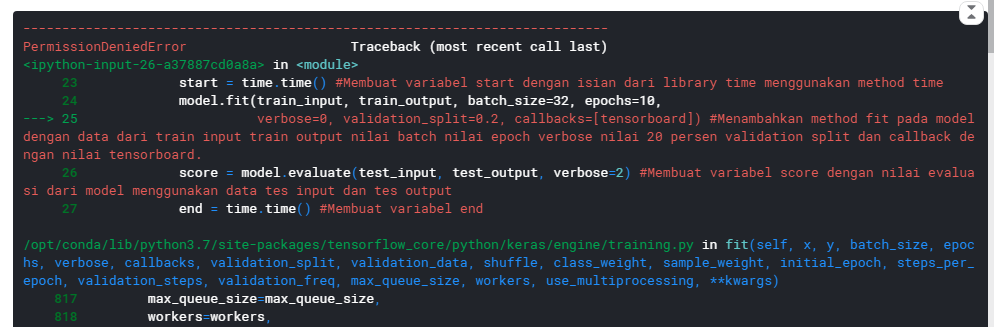
\includegraphics[width=10cm]{figures/1174076/figures7/error1.png}
		 \caption{Error}	
		\end{center}
	\end{figure}
	
	
	\subsubsection{Tuliskan kode eror dan jenis errornya}\hfill\\
		\begin{itemize}
		\item Permission denied
		
		
		\end{itemize}
	 
	\subsubsection{Solusi pemecahan masalah error tersebut}\hfill\\
		
	
\subsection{Link Youtube}
	
	\subsubsection{}\hfill\\
	